%导言区
\documentclass{ctexart}%ctexbook,ctexrep

%\usepackage{ctex}

%导言区:\usepackage{graphicx}
%语 法:\includegraphics[<选项>]{<文件名>}
%格 式:EPS,PDF,PNG,JPEG,BMP

\usepackage{graphicx}
\graphicspath{{figures/}}%图片在当前目录下(与代码要在同一个文件夹下)的figures目录,大括号实现分组

%正文区(文稿区)
\begin{document}
	\LaTeX{}中的插图:
	
	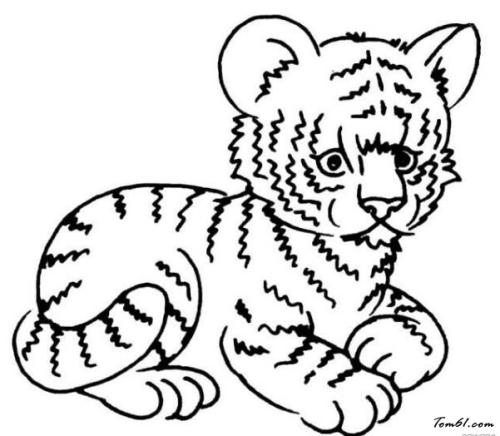
\includegraphics{lion}
	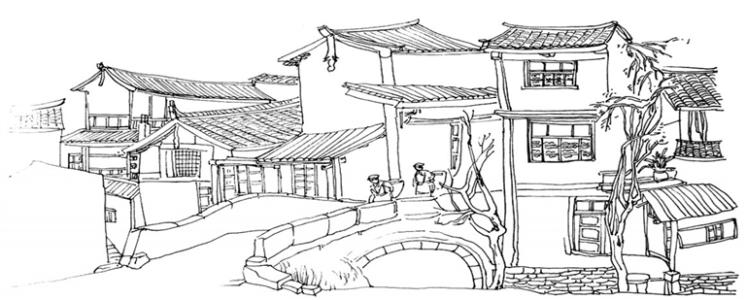
\includegraphics{mountain}
	
	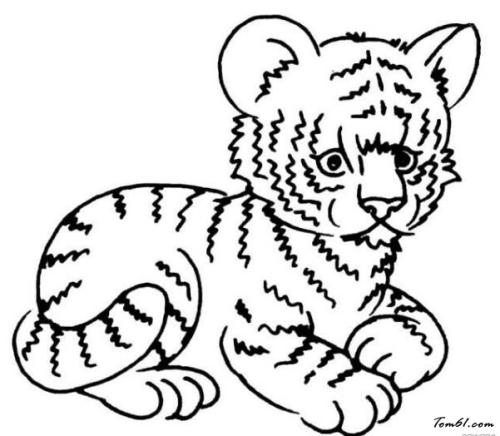
\includegraphics[scale=0.3]{lion}%设定缩放因子
	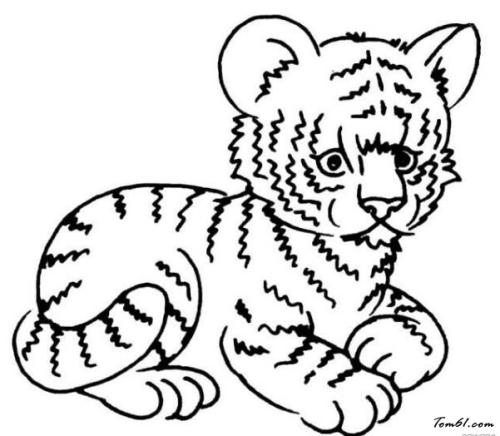
\includegraphics[height=5cm]{lion}
	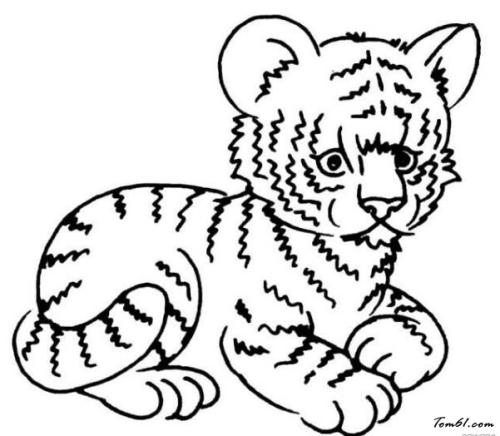
\includegraphics[width=2cm]{lion}\\
	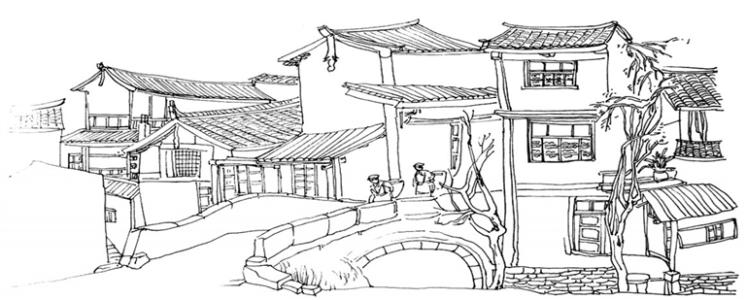
\includegraphics[scale=0.3]{mountain}%设定缩放因子
	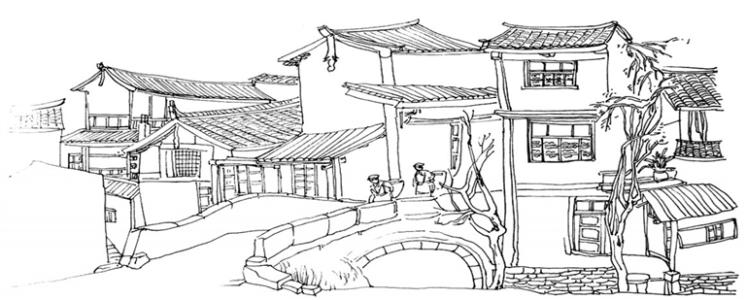
\includegraphics[height=3cm]{mountain}
	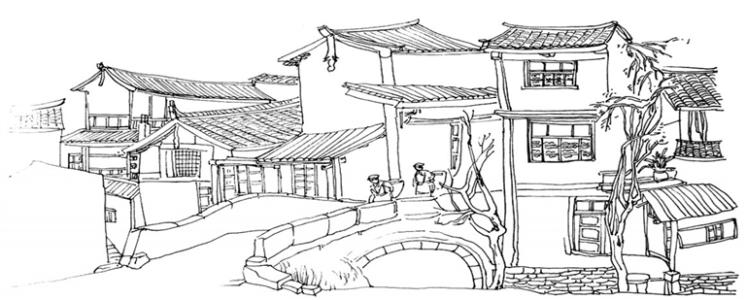
\includegraphics[width=5cm]{mountain}\\
	
	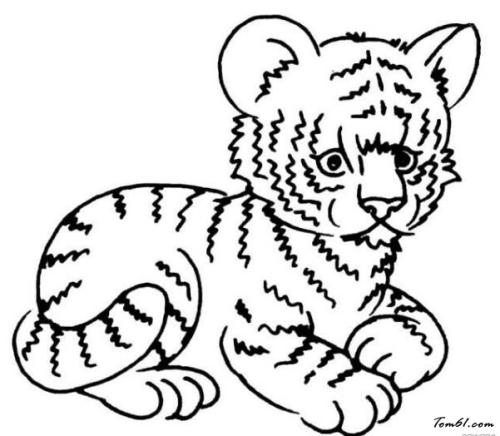
\includegraphics[height=0.6\textheight]{lion}\\%指定相对高度 文本版型的0.1倍
	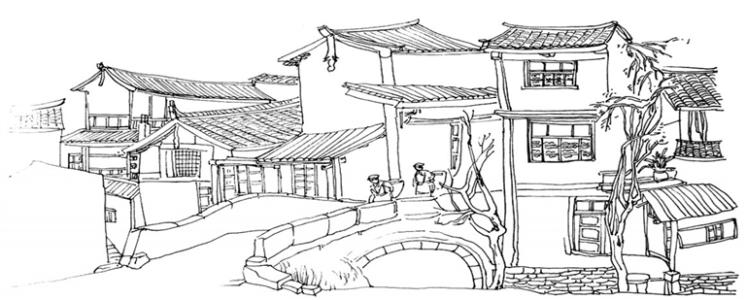
\includegraphics[height=0.6\textheight]{mountain}\\
	
	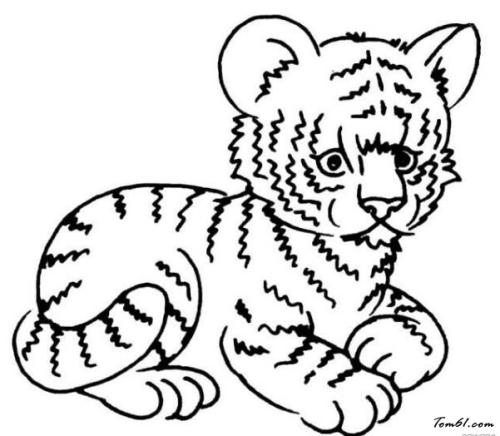
\includegraphics[width=0.2\textwidth]{lion}\\%指定相对宽度
	
	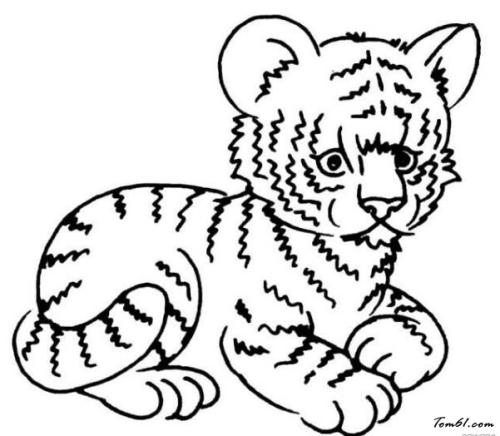
\includegraphics[angle=45,width=0.9\textwidth]{lion}%同时指定多个参数
\end{document}